%% LaTeX2e class for student theses
%% sections/main/2_requirements_engineering.tex
%%
%% Karlsruhe University of Applied Sciences
%% Faculty of  Computer Science and Business Information Systems
%%
%% --------------------------------------------------------
%% | Derived from sdqthesis by Erik Burger burger@kit.edu |
%% --------------------------------------------------------

\chapter{Requirements Engineering}
\label{ch:Requirements Engineering}

The main focus of this chapter is to describe the requirements that a reservation system for charging infrastructure needs to fulfill.
For that purpose, this work uses a fictional scenario to paraphrase and describe the underlying problem. Furthermore, a comprehensive representation of significant edge cases the system design has to consider is depicted as well as an accentuation of highlight potential problems is included.
Adapted from the requirements, use cases and goals are defined, giving an overview of the central tasks of this thesis.

\section{Scenario}
\label{ch:Requirements Engineering:sec:Scenario}

Beginning with the capture of fundamental points necessary for outlining the scenario, which represents the problem space the system is intended to operate.
The scenario includes, besides the location where the subsequent setting takes place, a group of personas describing fictional people representing actors, who interact with the system itself.
Each of these actors has different demands due to their current life situations regarding the usage of the system, which results in different expectations with respect to the fulfillment of their goals, based on the interaction with the system.
Formalizing these expectations and transforming them in a more general way, they could be derived as use cases separated by system actors for the implementation afterward.

\noindent To cover a broad range of possible users according to age, social backgrounds, and the ease of handling obstacles generated by new technologies, the scenario takes place in the context of the institution \acrfull{hka} located in the city of Karlsruhe.
As a partner of the \textit{Green4Ever} project \cite{noauthor_hka_nodate}, the \acrshort{hka} covers several aspects, which could be used for designing a sophisticated scenario. Aside from a broad range of users, ranging from students to the regular staff, it consists of multiple campus sites distributed all over the city.
This allows members of the institution to travel between the single sites and generate persistent demand for charging possibilities during the whole day.
Relevant for the description of the single actors, this scenario includes the sites \textbf{main campus}, \textbf{campus Amalienstraße}, also known as \textit{field office Amalienstraße}, and the \textbf{\acrfull{ltc}} with the amount of applicable \acrshortpl{cs}, which are listed in \ref{tab:campus-sites}.

\begingroup
\setlength{\tabcolsep}{10pt} % Default value: 6pt
\renewcommand{\arraystretch}{1.5} % Default value: 1
\begin{table}[h]
    \centering
    \caption{Campus sites and parking lots (site areas) in the \acrshort{hka} organization with the according number of available \acrshortpl{cs}.}
    \begin{tabular}{c|c|c}
        Site & Site Area & Number of \acrshortpl{cs} \\
        \hline
        Linder Technologie Campus & Private Parking Lot \acrshort{ltc} & 1 \\
        Linder Technologie Campus & Parking Lot \acrshort{ltc} & 3 \\
        Field Office Amalienstraße & Parking Lot Amalienstraße & 3 \\
        Main Campus & Parking Lot Steinbeishaus & 3 \\
    \end{tabular}
    \label{tab:campus-sites}
\end{table}
\endgroup

\noindent Furthermore, this work assumes the preferred way of movement to the sites is by public transportation or with their own cars.
As mentioned before, each of these campuses has its own parking lots equipped with a limited amount of \acrshortpl{cs} for students and the staff working at this site. Corresponding to the accessibility level declared in \ref{tab:cs-accessibility-levels}, the parking possibilities include public and semi-public charging opportunities.
Public parking lots and the corresponding \acrshortpl{cs} are available for students and staff members as well. In the case of semi-public parking lots, the access is only limited to visitors or staff exclusively. \\
Concerning the possibilities to configure \acrshortpl{cs}, all public stations are enabled for reservations. To prevent unnecessary complexity, this scenario does not include \acrshortpl{cs} without support for the reservation feature.
For administration and management of these facilities and the restricted charging resources, a software solution called \textit{Open e-Mobility} \cite{noauthor_github_nodate,noauthor_github_nodate-1,noauthor_github_nodate-3} is used, which includes a mobile application for the \acrshortpl{evu} and a web-based application for browser access, mostly used by administrative departments of the \acrshort{hka}. 
On behalf of these applications, the users have the possibility, according to their roles in the system listed in Table \ref{tab:system-role-collection}, to start or stop current charging sessions remotely or check for occupied \acrshortpl{cs} on the available sites and site areas.
Using privileged access via an administrative account, the user is able to deactivate or block connectors of specific \acrshortpl{cs}, to make them inaccessible until reactivation or a rebooting process.
By now, the administrator or the common user does not have the opportunity to reserve an available \acrshort{cs} connector in advance. Rather for themselves or on behalf of a specific user. This includes reservations for visitors arriving later or during times with high loads as well.
As an implication of this missing feature, a 'first-come-first-serve' mentality among the \acrshortpl{evu} was established, which led to decreased usage of \acrshortpl{ev} as a transportation means and an increasingly competitive behavior among the drivers.

\section{Stakeholders}
\label{ch:Requirements Engineering:sec:Stakeholders}

According to the scenario elaborated in Section \ref{ch:Requirements Engineering:sec:Scenario} above, the following groups of stakeholders could be identified. 
Considering the staff defined in \ref{ch:Requirements Engineering:sec:Stakeholders:ssec:Staff}, an additional decomposition into two subclusters is feasible for further differentiation. 
The description below provides an overview of the daily challenges members of these classes of people have to face in terms of the established implications defined by the scenario and their main objectives. 

\subsection{Student}
\label{ch:Requirements Engineering:sec:Stakeholders:ssec:Student}

Students represent the largest category of actors within the scenario and describe people studying at the \acrshort{hka}. Primarily, students spent most of their time on the \textbf{main campus} site, because the main part of lectures offered by the different faculties and the attendant exercises are located there.
In certain cases, some lecturers offer subjects at other campus positions, where doctoral research projects or research in general is outsourced. This involves several students each semester, commuting between the sites and generating additional demand on the existing charging infrastructure.
Due to the fact, that the number of students with \acrshortpl{ev} outnumbers the capacity of \acrshortpl{cs} at the different sites of the \acrshort{hka}, a student is typically concerned about the occupation rate of the public available \acrshortpl{cs}.
In consideration of planning their charging sessions, the students want an overview of available \acrshortpl{cs} at their campus site and want to reserve a public \acrshort{cs}, if they are available for reservation.
Therefore, they mostly rely on the mobile application offered by the institution, which serves as the main entry point for them to interact with the \acrshort{csms}. 

\subsection{Staff}
\label{ch:Requirements Engineering:sec:Stakeholders:ssec:Staff}

The staff of the \acrshort{hka} describes a group of people working at the institution, including roles like lecturers, cleaners, or librarians for example.
Based on their office location, they are typically assigned to one specific or several campus sites. Implicating the dedicated usage of the \acrshortpl{cs} for charging their \acrshort{ev}, available at their current working place.
In contrast to students, they have permission to access the \acrshortpl{cs} on the semi--public parking lots as well as the ones located in the public parking spaces. 
Due to the new home office regulations, staff members have the choice to work from home several days a week, which may relax the situation in regard to the high demand for charging infrastructure.
However, on office days staff members prefer to know the occupation rate of the \acrshortpl{cs} in the public or semi-public spaces and reserve a spot for a guaranteed charging possibility for their \acrshort{ev}.
Referring to the fact, that they spent most part of their daily working hours on the computer rather than their mobile, staff members utilize the web application as a primary way of managing their charging sessions.
The mobile application, the majority of the users rely on, is only used in certain cases.

\subsubsection{Maintenance Personal}
\label{ch:Requirements Engineering:sec:Stakeholders:ssec:Staff:sssec:Maintenance Personal}

As a dedicated subset of the regular staff working at the \acrshort{hka}, the maintenance personnel consists of caretakers in the first place. Their regular occupation consists of responsibility for the maintenance of the physical infrastructure as well as service offerings respecting the charging stations located on the different campuses.
For work--related trips between the single sites, the maintenance team makes use of a \acrshort{fev} with a dedicated \acrshort{cs} exclusively accessible by this vehicle and the respective staff.
To monitor the connected charging infrastructure and identify outtakes due to technical errors, the caretakers interact with the system using the administration dashboard, via a personal workstation in their office. In cases where a computer is not accessible, they utilize the mobile application to check the status of the charge points.
Besides the functionality as a supervisory system for the infrastructure, the caretakers need access to the reservations made on the \acrshortpl{cs} to resolve conflicts related to system outtakes or to manage the corresponding users.

\subsubsection{Administration}
\label{ch:Requirements Engineering:sec:Stakeholders:ssec:Staff:sssec:Administration}

Representing the administrative counterpart to the maintenance personnel, the group of secretaries working at the administration office manages internal data relating to staff and students belonging to the \acrshort{hka}, internal workflows, or communication with other organizations. 
This includes paperwork in relation to certain approvals for new students, maintaining the stored records, and processing incoming requests. Among other things, they are responsible for organizing events on and around the campus sites, planning upcoming visitations from external facilities, and coordinating the utilization and maintenance tasks for the charging infrastructure.
As a supervisory unit for the \nameref{ch:Requirements Engineering:sec:Stakeholders:ssec:Staff:sssec:Maintenance Personal}, they are scheduling maintenance and delegating tasks to the caretakers in case of extraordinary servicing.  
Therefore, staff members attending these positions need access to the \acrshort{csms} similar to the scope of the maintenance staff. In contrast to the caretakers, they are not leaving their office for interaction with the \acrshortpl{cs}, therefore they do not rely on the functionalities the mobile application has to offer.

\section{Personas}
\label{ch:Requirements Engineering:sec:Personas}

Appropriate to the defined stakeholders in the previous Section \ref{ch:Requirements Engineering:sec:Stakeholders}, each stakeholder requires a representation as a persona in regards to a dedicated user account in front of the system.
This allows a mapping between the accounts and the existing system roles, which enables easier separation between the use cases extracted later on and the assignment to the different stakeholders. 
Hereinafter, personas prescribing individuals inside the scenario including their dedicated demands in respect of the challenges their particular stakeholder group has to face. 

\begin{description}
    \item[Lisa Knaus] is a \nameref{ch:Requirements Engineering:sec:Stakeholders:ssec:Student} at the \acrshort{hka} and is studying computer science in the third semester. In respect of her current living situation, located in a village with limited access to public transportation, she primarily relies on driving by car as her main transportation means. 
    Fostered through financial benefits promoted by the different car manufacturers for young drivers with interest in acquiring an \acrshort{ev}, she sold her old car with \acrshort{ice} and switched to a \acrfull{fev}. 
    Under normal circumstances the health of the internal battery allows her to drive with a full charge from her hometown to the main campus site and back without a need to recharge. Occasionally she forgot to recharge at home and needed a charging possibility for her vehicle during the lecture time. Depending on the day and the utilization of the charging infrastructure, this is certainly a challenging task and she needs to arrive very early to get a free charging spot. 
    \item[Holger Starke] is an employee working as a member of the \nameref{ch:Requirements Engineering:sec:Stakeholders:ssec:Staff} at \acrshort{hka}. 
    Within the in-house server administration team, his daily tasks cover the maintenance of the server landscape, applying new versions of internal applications, and the creation of backups, securing the records of the internal user databases. 
    Thanks to the subsidies for electric vehicles from the state and his employer, he has bought a \acrshort{fev} and is using it as his main means of transport. 
    As compensation for the still missing charging possibilities at his apartment near the institution, he drives a short distance with his car every day, to use the existing charging infrastructure at the \acrshort{hka}, to recharge the batteries during working hours. 
    Therefore, he has to use the available \acrshortpl{cs} at the different campus locations without any guarantee to recharge. 
    With the increasing amount of students and coworkers arriving with \acrshortpl{ev} over time, the search for a free \acrshort{cs} becomes more and more demanding. 
    Especially scheduled service work later in the day, located at other campuses, emerge to a running the gauntlet for parking lots with \acrshortpl{cs} equipped. 
    \item[Dieter Krause] is engaged in the role of a caretaker as part of the \nameref{ch:Requirements Engineering:sec:Stakeholders:ssec:Staff:sssec:Maintenance Personal} at \acrshort{hka}. During his previous position, he acted as a carrier for the daily book orders for the students at the university library on the main campus site. 
    For the reduction of \acrshort{co2} the \acrshort{hka} bought a \acrshort{fev} for bridging the short distances between the various libraries within the city. 
    This confronted him with the according up- and downside of driving an \acrshort{ev} in a very early stage. 
    Missing charging opportunities and insufficient battery life were only two obstacles he had to bother with, every day. 
    This led him to the conclusion to switch positions and he took over the responsibility for the charging infrastructure maintenance and management on the campus sites to improve the situation for all involved parties. 
    Alongside the continuously increasing number of \acrshortpl{cs}, he has fostered the establishment of dedicated charging possibilities for the members of the \nameref{ch:Requirements Engineering:sec:Stakeholders:ssec:Staff} and introduced an exclusive \acrshort{cs} for the \acrshortpl{ev} of the \nameref{ch:Requirements Engineering:sec:Stakeholders:ssec:Staff:sssec:Maintenance Personal}. 
    Even on days with a high emergence of student vehicles on the public parking lots, he and his colleagues could recharge the batteries of their \acrshortpl{fev}. 
    \item[Nadine Funke] acts as a secretary in the \nameref{ch:Requirements Engineering:sec:Stakeholders:ssec:Staff:sssec:Administration} office at \acrshort{hka}. Formerly she worked at the public administration office in Karlsruhe, in the area of public parking spaces, where she had her first experience with the problems concerning the management of the charging infrastructure on public parking lots. 
    For this reason, she does not drive an \acrshort{ev} herself and uses public transportation instead. In contrast to her previous position at the public administration office, the tasks regarding the management of the \acrshortpl{cs} are, thanks to the introduced system, much more convenient and do not require a lot of manual work. 
    By accessing the \acrshort{csms} dashboard, she could filter for the wanted \acrshort{cs} and have all the information in one place. 
    However, blocking \acrshortpl{cs} for upcoming visitors is, despite the new system, still a huge overhead for the secretaries at the \acrshort{hka}. 
    Up to now, she has had to select the specific \acrshort{cs} and the corresponding connector to block it, and she has to unblock it again when the guest has arrived.
\end{description}

\section{Role Mapping}
\label{ch:Requirements Engineering:sec:Role Mapping}

To distinguish between the single users and their privileges in compliance with the range of associated functionalities, the system introduces a set of roles. Besides the role of the basic user, two variations of administrators and a user for demo purposes are provided.
For a better understanding of these privileges and their purpose inside the system, the following table \ref{tab:system-role-collection} lists the relevant roles, their system shortages, and a brief explanation.

\begingroup
\setlength{\tabcolsep}{10pt} % Default value: 6pt
\renewcommand{\arraystretch}{1.5} % Default value: 1
\begin{table}[h]
    \centering
    \caption{Role collection provided by the system.}
    \begin{tabular}{c|c|c|m{6cm}}
        Role & System & Shortage & Description \\
        \hline
        Basic & \verb|BASIC| & \verb|B| & Standard user without administrative privileges \\
        Admin & \verb|ADMIN| & \verb|A| & User with administrative privileges inside one organization \\
        Site Admin & \verb|BASIC| & \verb|B| & User with administrative privileges for assigned sites \\
        Site Owner & \verb|BASIC| & \verb|B| & User with administrative privileges for owned sites \\
        Super Admin & \verb|SUPER_ADMIN| & \verb|S| & User with extended administrative privileges for the management of organizations and tenants \\
        Demo & \verb|DEMO| & \verb|D| & Demo user with predefined login data, primarily used for demonstration purposes
    \end{tabular}
    \label{tab:system-role-collection}
\end{table}
\endgroup

\noindent Based on the available user privileges introduced in Table \ref{tab:system-role-collection} and provided by the system out of the box, the next step is the mapping of the created personas, established in Section \ref{ch:Requirements Engineering:sec:Personas}, to their corresponding role inside the system.
The criteria for the assignment are primarily based on the tasks the single users have to fulfill and with respect to their position inside the scenario. \\
\noindent The role mapping proposed in the context of this work is presented below:

\begin{figure}[h]
    \centering
    \begin{tikzpicture}
      [
        group/.style={ellipse, draw,inner sep=-2pt,minimum height=50pt,minimum width=30pt},
      ]
      \node (b) at (0,4) {Basic};
      \node (d) at (0,3) {Demo};
      \node (a) at (0,2) {Admin};
      \node[align=center] (s) at (0,1) {Super Admin};
      
      \node (student) at (4,4) {Student};
      \node (staff) at (4,3) {Staff};
      \node[align=center] (mp) at (4,2) {Maintenance\\Personal};
      \node (admin) at (4,1) {Admin};
      
      \foreach \i/\j in {a/mp,a/admin,b/student,b/staff}
        \draw [->, shorten >=2pt] (\i) -- (\j);
      \node[fit=(a) (b) (s) (d), group,label={left:{\textbf{Roles}}}] {};
      \node [fit=(student) (staff) (mp) (admin), group,label={right:{\textbf{Groups}}}] {};
    \end{tikzpicture}
    \caption{Mapping of the roles to the group identified in the scenario described in \ref{ch:Requirements Engineering:sec:Scenario}.}
    \label{fig:role-mapping}
\end{figure}


% \begin{align*}
%     Basic &= \bigl\{\ Student,\ Staff\ \bigr\},\\
%     Admin &= \bigl\{\ Maintenance\ Personal,\ Administration\ \bigr\}
% \end{align*}

\newpage

\section{Goals}
\label{ch:Requirements Engineering:sec:Goals}

Based on the scenario and the corresponding stakeholders, the relevant goals for the resulting implementation are prescribed. As part of this work, a goal is handled as a requirement, the final product has to fulfill. 
Taking into account the different wishes in terms of the situations in which the respective stakeholders interact with the system, the following objectives could be defined.

\noindent \textbf{Goal 1 - Management Capabilities} As a major concern of this work the designed system, should serve as a central point for management purposes of the registered \acrshortpl{cs}. This should provide a basic set of functionalities covering specific administration tasks tailored for a certain group of users. 
Besides role mapping according to a subset of functions, the system should detect unintended usage and prohibit breach of privileges.
Furthermore, the involved users will be provided with all relevant information by the system and know their current position within the different phases of the processes at each time. 

\noindent \textbf{Goal 2 - Self-Healing and Autonomous Processes} In case of invalid user input or violation of predefined constraints inside the processes, the system should provide mechanisms for self-healing and autonomous error handling. 
In addition to increased consistency of data within the underlying database, the ease of use of the system should be a positive side effect.

\noindent \textbf{Goal 3 - Support of relevant standards} Considering the implementation of relevant communication protocols and the interoperability between different systems of \acrshortpl{cs}, \acrshortpl{ev} and \acrshortpl{csms}, the system should support well-established standards for communication and data exchange in the context of \acrshort{emobility}. 
Alongside the standards like \acrshort{ocpp} or \acrshort{ocpi}, described in the subsection \ref{ch:Fundamentals:sec:Electric Mobility:ssec:Relevant Standards}, other alternatives exist in the further evolving industry with different targets in mind. 
Considering the already implemented standard inside the underlying product, the \nameref{ch:Fundamentals:sec:Electric Mobility:ssec:Relevant Standards:sssec:OCPP} should be the protocol for the communication between \acrshort{cs} and \acrshort{csms}.

\noindent \textbf{Goal 4 - Modular Design} In addition to the previously mentioned goals that focus on the implemented functionality, the architectural design of the software itself should also be considered. 
As part of a system that follows both a monolithic and a microservice-based approach, multiple services interact simultaneously alongside each other. The implementation and software architecture of this work aim to avoid compromising existing functionality through poor design choices or neglected separation of concerns. 
Preferably, the new functionality should be encapsulated as part of a module, which separates the system based on its responsibilities according to the definition in \cite{clements_documenting_2011}. This should ensure easier extensibility of existing features and allow convenient maintainability.

\section{Use Cases}
\label{ch:Requirements Engineering:sec:Use Cases}

The use cases illustrated in the use case diagram in \ref{fig:use-cases} were elaborated based on the goal definitions in the previous Section \ref{ch:Requirements Engineering:sec:Goals} and the stakeholder requirements from Section \ref{ch:Requirements Engineering:sec:Stakeholders}.
Typically, software development processes such as \acrshort{rup} \cite{kruchten_rational_1999} differ between the groups of stakeholders who have an interest in the resulting product and the actors who are actually interacting with the real system. 
As part of this scenario, the stakeholders actually represent the actors used for defining the use case in regard to interacting with the system.
The main use case, as highlighted by \textbf{goal 1}, involves managing and administering reservations within the reservation system. This encompasses creating, modifying, viewing, and deleting existing reservations made either by the users themselves or on their behalf by the administrator.
Corresponding to \textbf{goal 2}, the \textit{Scheduler} entity facilitates the required self-healing procedures. This necessitates the system to communicate with itself and employ background processes to manage forthcoming, current, and expiring reservations.
Apart from the primary focus on non-functional requirements related to \textbf{goals 3} and \textbf{4}, an additional functional requirement with reference to the selective activation and deactivation of the reservation module could be identified.
The privileges for maintenance and configuration of the particular organizations, represented as tenants inside the system, are part of the \verb|SUPER_ADMIN| role.
Usually, an external service provider outside the customer organizations is responsible for determining the scope of operation, for the service offerings provided to its customers. This role is referred to as \verb|SUPER_ADMIN|. As there is no direct interaction with the system in terms of the reservation process, there is no dedicated actor assigned to this role within the above scenario.
For comprehensively addressing all the aspects mentioned in the set goals, it is necessary to include this role with its corresponding functionality when defining the required features.

\begin{figure}[h]
    \centering
    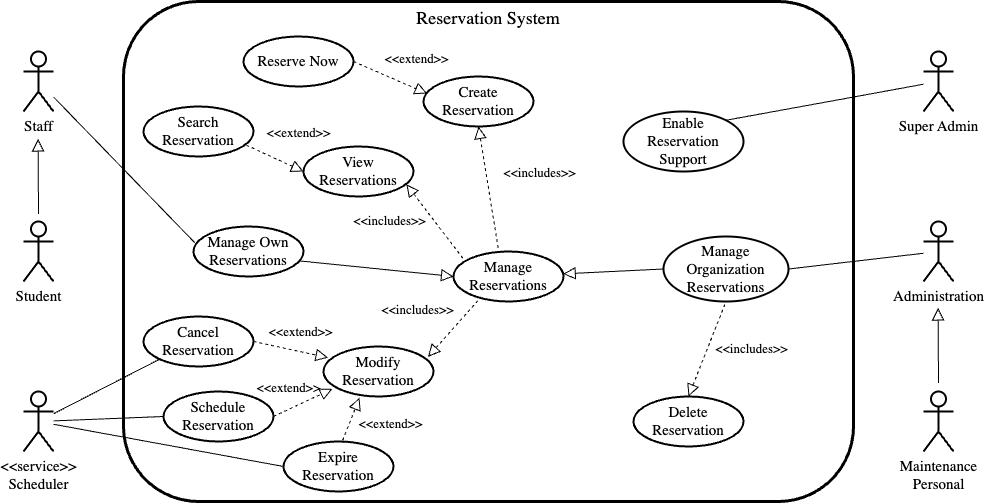
\includegraphics[scale=0.4]{resources/images/main/2_requirements_engineering/UseCases.png}
    \caption{Use Cases considering the stakeholders of the reservation system.}
    \label{fig:use-cases}
\end{figure}
